\chapter{Methodologies: Design and Implementations}\label{ch:methodologies}
This chapter will explore the design and implementation of the Arabic Dialect identification System. 
As well as the base dataset choice, it's preparation and preprocessing. The experiments conducted throughout 
this thesis will be briefly introduced and Chapter \ref{ch:experiment} will further explore them in detail. 
The code used, the dataset design and results are publicly available on the GitHub repository 
\url{https://github.com/madelineyounes/thesis}. 


\section{Dataset}\label{sect:dataset}
The dataset to be used in this thesis is the \textbf{ADI17} dataset \cite{shon_adi17_2020}. The \textbf{ADI17} dataset consists of audio segments from known Youtube videos with dialects from 17 different Middle Eastern and North
African countries. The dataset is divided into training, development and test data groups. The training set contains 
3000hrs of audio total while the development and test combined is 57hrs of audio. The specifics of the dataset can be seen in Figure \ref{fig:ADI17}.
The data was collected from around 30 different Youtube channels per country and the primary dialect each Youtube channel used was verified by a human annotator. Using the Youtube channel's 
dialect audio segment's dialectal label was allocated. The training data relies on this for its labelling, whilst 
the test and development data was annotated by a human annotator. The audio segments are split into utterances ranging from 10-20s in length, which are small portions  
of audio generated by segmenting the original audio at silence points. These silence points are usually natural pauses in conversation and a threshold 
is used to determine how long the silence must be before the audio is split. The creators of the ADI17 dataset have not specified the threshold that they used. 
The dataset is labelled using 17 regions, a portion of this thesis explores creating a generalised DID of 4 generalised umbrella dialects that encompass this finer set of regional dialects as shown in Figure \ref{fig:DialectSplit}. 
Hence, the of data from each region is taken to construct the training set for the generalised dialects as shown in Figure \ref{fig:ADI17}. 
The core challenges with the ADI17 dataset are that the acoustics are unbalanced across each of the dialect regions and the amount of data provided is unbalanced. The amount of noise in each of the 
regions datasets is shown in Figure \ref{fig:noiseDataSet}, although its effect on the DID will be mitigated through using channel normalisation and filtering experimented with, as the papers \cite{boril_arabic_2012,pohjalainen_spectral_2016} have shown is effective at increasing 
accuracy of Arabic DIDs. The dataset is also unbalanced in terms of amount of training data for each region as shown in Figure \ref{fig:ADI17}, with Jordan having the least amount of data. To ensure that 
training, validation and testing is balanced between all the dialects only a subset of the dataset is used. 

A script was written to generate three csv files (test, training and validation) containing the file names and the dialectal label of each file. 
For the umbrella DID, the script would ensure that equal amounts of files were taken from each regional dialect and then changed the label from the regional one 
to it's corresponding umbrella dialect. eg. for the umbrella DID test csv 700 files were allocated to the North African umbrella dialect, 175 were from each of the regional dialects (DZA, MAR, MRT, LBY). 
Within the system pipeline 70\% of the data is allocated to training, 20\% to validation and 10\% to test. A breakdown of this for both the umbrella DID and the regional DID is shown in tables \ref{tab:umbrsplit} and \ref{tab:regsplit}
respectively. 

\begin{figure}[h!]
    \centering
    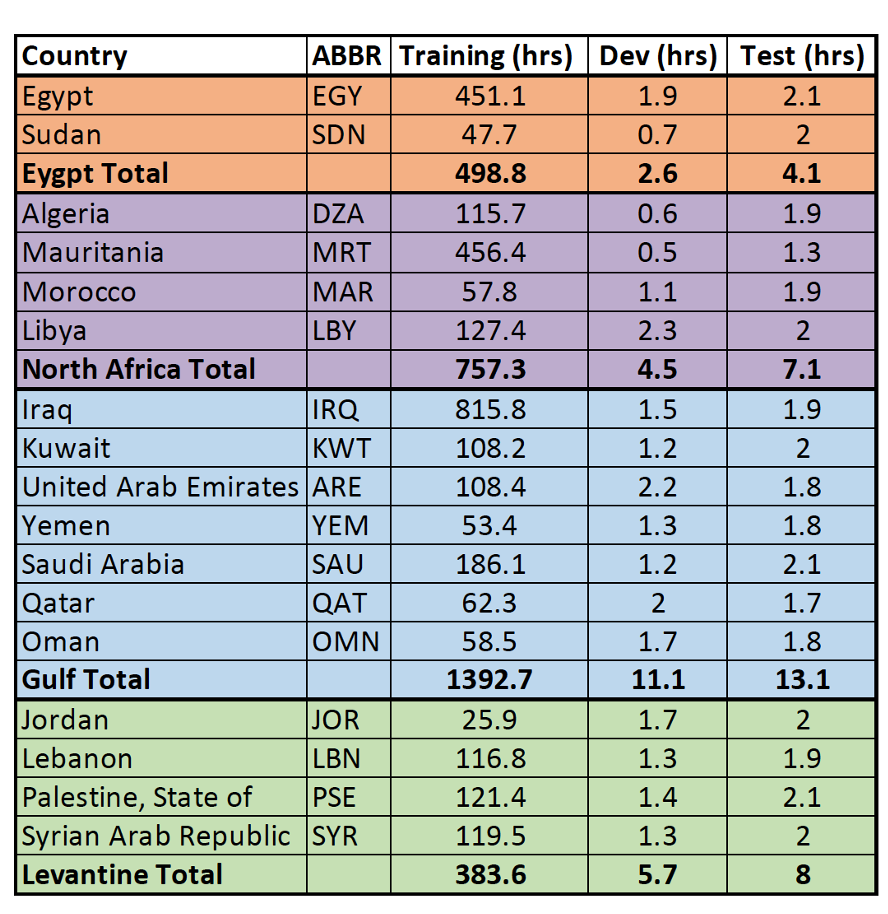
\includegraphics[height=10cm]{ADI17data.png}
    \caption{ADI17 Dataset Details.}
    \label{fig:ADI17}
\end{figure}

\begin{figure}[h!]
    \centering
    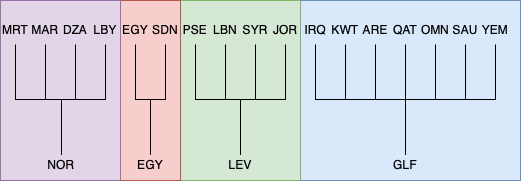
\includegraphics[height=4cm]{ArabicDialectGroups.png}
    \caption{Regional to Umbrella Dialect Grouping.}
    \label{fig:DialectSplit}
\end{figure}

\begin{figure}[h!]
    \centering
    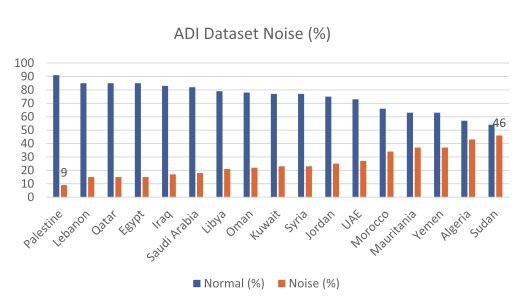
\includegraphics[width=\textwidth]{noiseDataset.png}
    \caption{ADI17 Dataset Noise levels. \cite{alhakeem_confidence_2021}}
    \label{fig:noiseDataSet}
\end{figure}

\begin{table}[h!]
    \begin{tabular}{|llll|}
    \hline
    \multicolumn{4}{|l|}{Umbrella DID File Breakdown}                                                                            \\ \hline
    \multicolumn{1}{|l|}{}           & \multicolumn{1}{l|}{Split (\%)} & \multicolumn{1}{l|}{Number of Files} & Total Time (hrs) \\ \hline
    \multicolumn{1}{|l|}{Training}   & \multicolumn{1}{l|}{70}         & \multicolumn{1}{l|}{2800}            & 7.78             \\ \hline
    \multicolumn{1}{|l|}{Validation} & \multicolumn{1}{l|}{20}         & \multicolumn{1}{l|}{800}             & 2.22             \\ \hline
    \multicolumn{1}{|l|}{Test}       & \multicolumn{1}{l|}{10}         & \multicolumn{1}{l|}{400}             & 1.11             \\ \hline
    \end{tabular}
    \caption{Table showing the file breakdown for the Umbrella DID pipeline.}
    \label{tab:umbrsplit}
\end{table}

\begin{table}[h!]
    \begin{tabular}{|llll|}
    \hline
    \multicolumn{4}{|l|}{Regional DID File Breakdown}                                                                            \\ \hline
    \multicolumn{1}{|l|}{}           & \multicolumn{1}{l|}{Split (\%)} & \multicolumn{1}{l|}{Number of Files} & Total Time (hrs) \\ \hline
    \multicolumn{1}{|l|}{Training}   & \multicolumn{1}{l|}{70}         & \multicolumn{1}{l|}{11900}           & 33               \\ \hline
    \multicolumn{1}{|l|}{Validation} & \multicolumn{1}{l|}{20}         & \multicolumn{1}{l|}{3400}            & 9.4              \\ \hline
    \multicolumn{1}{|l|}{Test}       & \multicolumn{1}{l|}{10}         & \multicolumn{1}{l|}{1700}            & 4.72             \\ \hline
    \end{tabular}
    \caption{Table showing the file breakdown for the Regional DID pipeline.}
    \label{tab:regsplit}
\end{table}
\pagebreak
\section{Implementation of Arabic DID System}\label{sect:impDID}
This section will describe the implementation of the system in Python. The pipeline scripts leverage 
the Hugging Face Transformer library but expand out the Dataset, DataLoader and Trainer classes rather than only using 
their default functionality. The pretrained models are also imported using this library. 

\subsection{Overall System Design}

The proposed pipeline design for the Arabic DID is illustrated in Figure \ref{fig:sysOverview}. The system takes in three csv files, training, validation and test. The files specify the labels and file paths 
of the audio files.  There is a corresponding dataloader for each set which manages the processing of the 
audio files. It extracts the audio features, trims the audio to a specified length, normalises them, then shuffles and groups the data into 
batches. The Experiment \ref{sect:noiseExp} also tests filtering the data to remove noise. The main portion of the pipeline is the trainer, which manages the fine-tuning of the pretrained model. 
The model is prepared to be trained at the start of the pipeline with the layers to be trained unfrozen. In all the experiments 
the feature projector layer and the linear classifier layer are unfrozen. In the experiment \ref{sect:encoderExp} unfreezing and training 
the encoder layers is explored. While in experiment \ref{sect:downExp} a downstream model is inserted into the network, this is discussed further in Section 
\ref{sec:down}. At each epoch the processed training data is passed through the model calculating the loss, using a cross entropy loss function 
then updating the layer weights accordingly. The model is then put in evaluation mode, to assess the accuracy at that epoch using the validation dataset. 

Once a model is fine-tuned it is then run through a third set of data which has not been used in the training process. Similarly to 
the main pipeline, the audio features are extracted from the audio file, it is truncated, batched and then fed into the final model. The Python package 
sklearn.metrics is then given the predictions and true labels to generate the confusion matrices and classification report. A function was written taking advantage of the matplotlib.pyplot
library to convert the confusion matrices into colour map plots.  This testing pipeline is shown in the Figure \ref{fig:testPipe}.

\begin{figure}[h!]
    \centering
    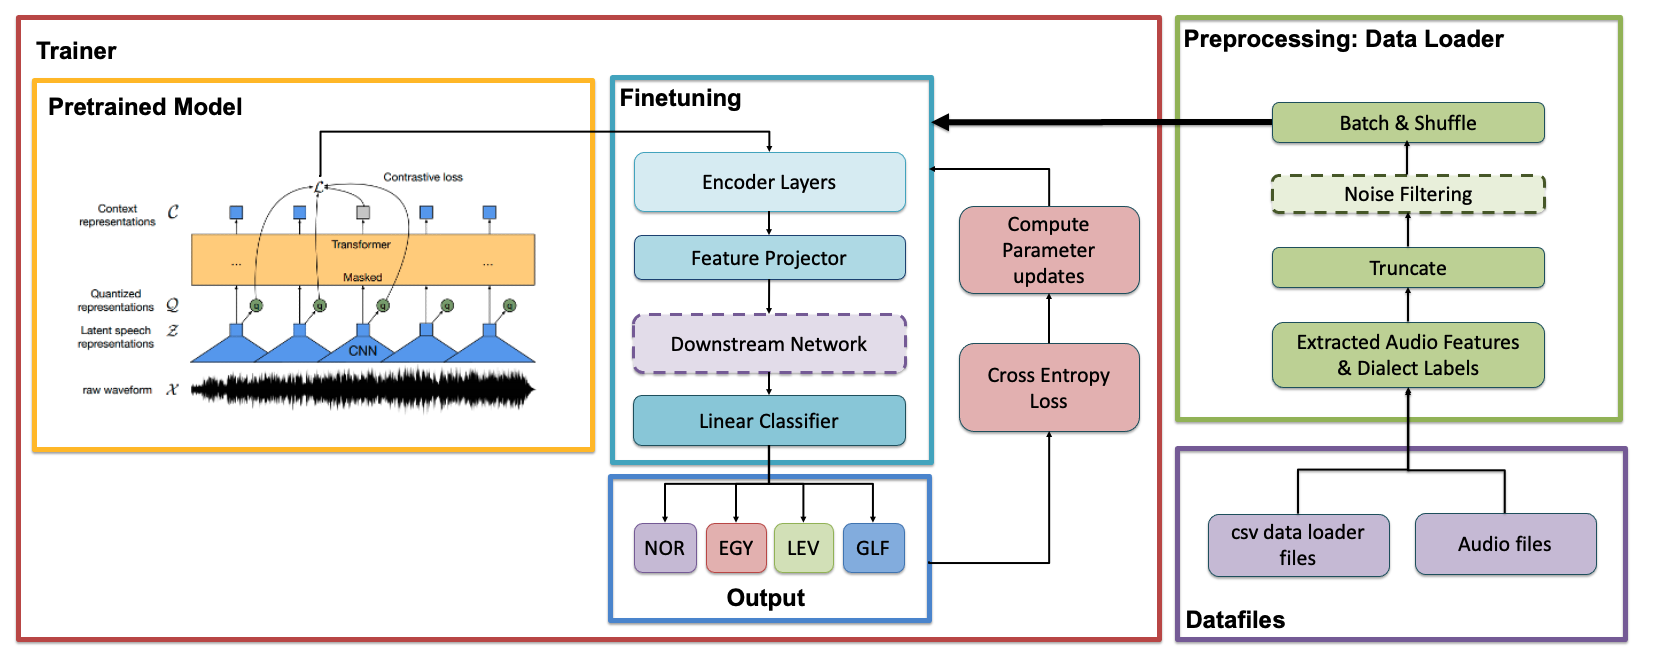
\includegraphics[width=\textwidth]{diagrams/systemOverview.png}
    \caption{Overview of the System.}
    \label{fig:sysOverview}
\end{figure}

\begin{figure}[h!]
    \centering
    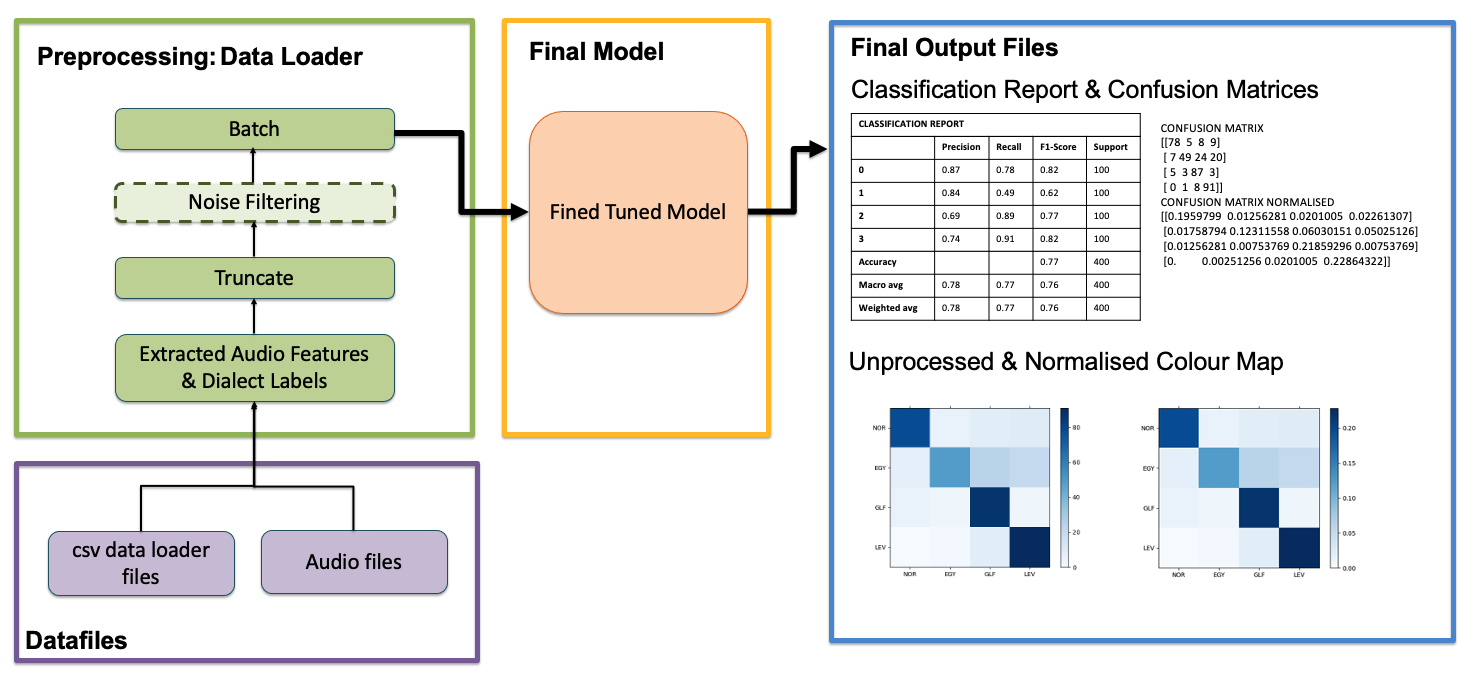
\includegraphics[width=\textwidth]{diagrams/testPipeline.png}
    \caption{Test Pipeline.}
    \label{fig:testPipe}
\end{figure}
\pagebreak
\subsection{Pre-training}
All the pre-trained models used in this thesis were trained by Facebook using 16kHz sampled speech audio and were imported from the Hugging Face Transformer library. The advantage of using a pretrained 
model is the significant amount of resources needed to sufficiently train a wav2vec 2.0 or hubert architecture is not required. 
Several model choices were explored, they are listed with a summary of their key features in the Table \ref{tab:PretrainedModels} and their performance
was tested in Experiment \ref{sect:pretrainExp}. 

\begin{table}[hb!]
    \label{tab:PretrainedModels}
    \begin{center}
    \begin{tabular}{|m{3cm} || m{7cm} | m{6.5cm} |}
        \hline
        \textbf{Model} & \textbf{Key Features} & \textbf{Hugging Face Path}\\
        \hline
        Hubert & 
        \textbf{Training:} 960 hrs of English unlabeled speech and 1hr of labelled speech from  Librispeech corpa (LS-960).\newline 
        \textbf{Structure:} Masked hidden units.
        & facebook/hubert-base-ls960\\
        \hline
        wav2vec 2.0 & 
        \textbf{Training:} 960 hrs of English unlabeled speech and 1hr of labelled speech from Librispeech corpa (LS-960). \newline
        \textbf{Structure:} Masking and contrastive based learning.
        &facebook/wav2vec2-base\\
        \hline
        XLS-R &
        Fined tuned version of wav2vec 2.0.\newline
        \textbf{Training:} 56k hrs unlabeled speech data \newline in 53 languages, from Multilingual \newline LibriSpeech (MLS), 
        Babel and Common Voice speech corpses. 
         &facebook/wav2vec2-large-xlsr-53\\
        \hline
        XLS-R Arabic & XLS-R variant finetuned on 7.5hrs of male voiced Syrian (Levantine) Arabic with a Damascus accent &
        elgeish/wav2vec2-large-xlsr-53-arabic \\
        \hline
        wav2vec sid & wav2vec 2.0 variant finetuned for the downstream task of speaker identification using the VoxCeleb1 corpa. 
         &superb/wav2vec2-base-superb-sid\\
        \hline
        wav2vec lid & wav2vec 2.0 variant finetuned for\newline the downstream task of\newline language identification.
        &log0/wav2vec2-base-lang-id\\
        \hline
    \end{tabular}
    \caption{Summary of the pretrained models used in this thesis.}
    \end{center}
\end{table}

\subsection{Fine-tuning}
Fine-tuning is the process which adapts the pretrained model to the downstream task of Arabic dialectal identification. 
The pretrained model is initialised with the weights from in its initial training and the final classification layer or downstream network is randomly initialised. 
So, for the umbrella DID the output of the final layer is 4 and for the regional DID is 17, corresponding to the number of classes each DID have. In the Experiment {} 
the CNN encoder layers are unfrozen, so that their weights are also updated. 

The meta-paramaters of the trainer are kept consistent for each of the experiments. The learning rate is set to 0.00004, an Adam optimiser is used with a learning rate warm-up for the first 
10\% of updates. The updates are then linearly decayed for the remainder of the updates. A batch size of 40 per GPU is used thereby when using 2 GPUs the samples processed at one time is 80 and 
in the case where 3 GPUs are used 120 samples are processed. 

Training is performed on the shared UNSW computational cluster Katana[] using 2 to 3 Tesla V100-SXM2 32GB GPUs depending on the experiment being conducted and it's reasource requirements. 
\subsection{Downstream Network}\label{sec:down}
When using transfer learning, for some downstream tasks it can be advantageous to add a network to the structure of a pretrained model, this structure is referred to as a downstream model. 
To investigate the effectiveness of a downstream model on creating an Arabic DID, a downstream model is inserted into the wav2vec 2.0 architecture. 
The model is inserted between the Feature Projector layer, taking in the 256 outputs from it and the final linear layer with the classifier classes. 
For experiments with a downstream model the weights of a previously successful model are imported onto the head of the model. The pretrained model head is then 
frozen and only the downstream model with the final linear classifier layer is trained. This thesis tested DNN and LSTM model structures. 
For the DNN downstream network the number of layers within the model is varied between 3 and 6 layers. 
The DNN networks are comprised of rectified linear activation function (ReLu) layers. The ReLu layers are a linear piece wise function that outputs the input if it is given a positive value and zero if it isn't. 
It was chosen to be used in the DNN structures as they are one of the most common activation functions, relatively simple to train and achieve high performances with. Whilst the 
LSTM architecture is constructed with a Long short-term memory (LSTM) layer that uses information from past and current data samples, a dropout layer which reduces overfitting by randomly setting the inputs to 0 and 
the softmax layer converts the inputs into probabilities. All the downstream model structures explored are shown in Figure \ref{fig:downModel}, in this figure the number of classes is set to 4 for the umbrella DID. 

\begin{figure}[h!]
    \centering
    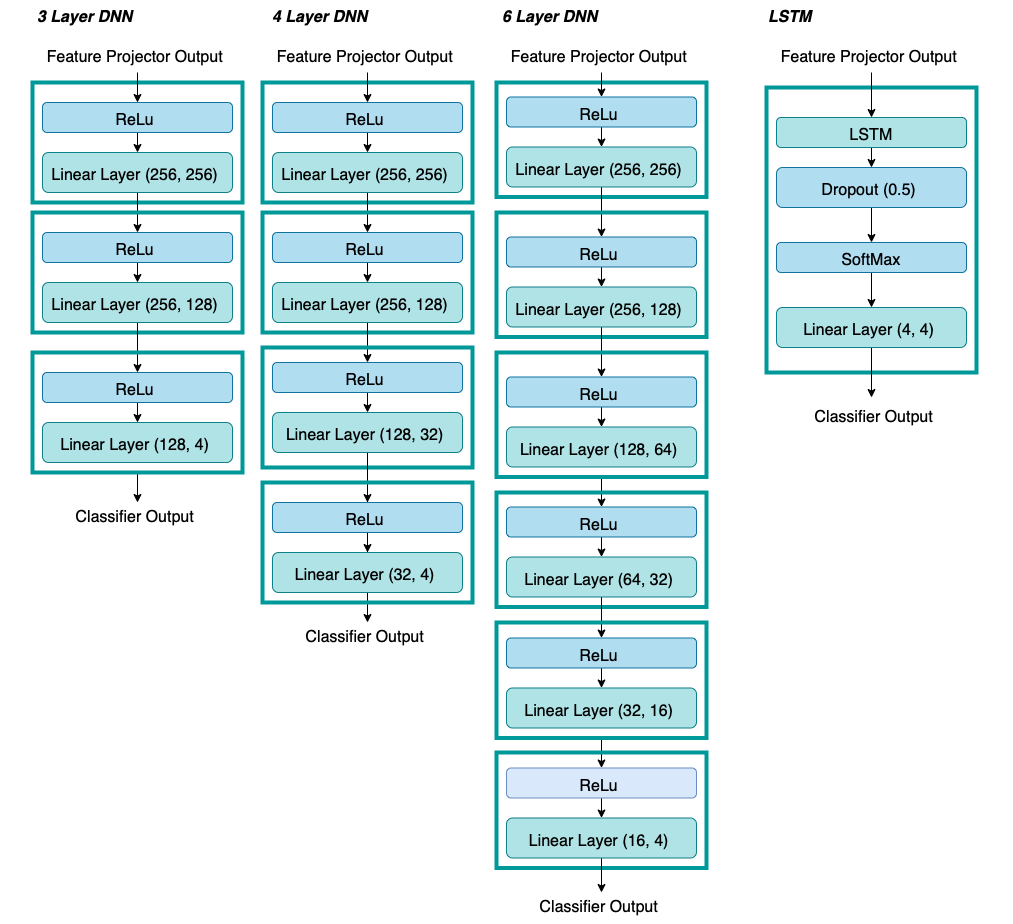
\includegraphics[width=\textwidth]{diagrams/downstreamModel.png}
    \caption{Downstream model structures.}
    \label{fig:downModel}
\end{figure}